\chapter{Measurements}\label{chap:measurements}
In the previous section, we described the effects of a system coupled to its environment. In most cases the interactions of our system is unwanted, but in one case it is necessary: readout. Without interacting with the system, there is no way to gather information about it. Often measurements are portrayed as instantaneous and projective. In reality, it is not instant. In this chapter, we will introduce the idea of a generalized measurement using a Positive Operator-Value Measure and see how this effects the evolution of a state. This will allow us to modify the master equation to include terms representing backaction and correlate that with our measurement record. Finally we will see how the dynamics of a qubit/resonator system is altered during measurement. Most of this chapter is based on the excellent introduction to continous quantum measurements by Jacobs and Steck \cite{jacobs_straightforward_2006}.

\section{Generalized Measurement}
When one first encounter quantum mechanics, a measurement is an instantaneous and complete projection of a state onto the measured quantity. Measuring an observable given by the hertmitan operator in its eigenbasis, $\mathcal{O} = \sum_n O_n \ket{n}\bra{n}$ (with $\ket{n}$ the eigenstates of O) would thus result in a projection of a state $\ket{\psi}$ onto the state $\ket{n}$ with probability $|\braket{n}{\psi}|^2$. In our measurement record, we would find the corresponding value $O_n$. \footnote{In the formalism of density matrices the probability is $\mel{n}{\rho}{n}$ and the projected state would be $\ket{n}\bra{n}$.} This is indeed a possible measurement, but this \textit{von Neumann} measurement is just a small set of possibilities which can not explain what happens if we only extract partial information from the system. We will here describe a more general description of measurements. 
% Furthermore, if we want to measure the I-quadrature, a contious variable, it would be tough to do with a delta function. Therefore, we also need a framework, which represents contious measurements. \todo{Clean up this transition}\todo{The content of this section is based on the excellent review of continuous measurement by Jacobs and Stech \cite{straightforward_introduction}} 

\subsection{Positive Operator-Valued Measure (POVM)}
If we were to start with a state $\rho$ and perform a von Neumann measurement with the projection operator $P_n = \ket{n}\bra{n}$, we will get:
\begin{equation}\label{eq:projection_measurement}
    \rho_f = \ket{n}\bra{n}= \frac{P_n \rho P_n}{\Tr(P_n \rho P_n)}, \text{with probability: } \Tr(P_n \rho P_n) = \rho_{nn}
\end{equation}
In describing this projection, we often consider the output $n$ with probability $\rho_{nn}$ but not always recognize that it equally gives us the value $\neq n$ with probability $1 - \rho_{nn}$. In this case the state will be proportional to $\rho_f \propto \rho - \rho_{nn}\ket{n}\bra{n}$. If we were to also represent this with an operator $P_{\text{not n}} = \identity - P_n$, we could think of the measurement as applying  a set of the operators $\{P_n, P_{\text{not n}}\}$ and applying the operator depending on the outcome.

By expanding this set from two to more operators, we can generalize measurements. The generalization comes as a set of operators $\{\Omega_m\}$ that satisfy:
\begin{equation}\label{eq:sum_requirement_POVM}
    \sum_m \Omega_m^\dagger \Omega_m = \identity
\end{equation}
Applying an operator from this set alter the state according to ( \ref{eq:projection_measurement}):
\begin{equation}\label{eq:POVM_collapse}
        \rho_f = \frac{\Omega_m \rho  \Omega_m^\dagger}{\Tr(\Omega_m \rho \Omega_m^\dagger)}, \text{with probability: } \Tr(\Omega_m \rho \Omega_m^\dagger)
\end{equation}
Here we are allowed to combine multiple measurements into one question. An example could be, what is the probability of measuring the operator in an interval $m\in[a, b]$. This will of course just be sum of probabilities: 
\begin{equation}
    P(m \in [a, b]) = \sum_{m = a}^b \Tr(\Omega_m\rho\Omega_m^\dagger)
\end{equation}
Or rearranging using linearity and cyclic properties of the trace:
\begin{equation}
    P(m \in [a, b]) = \Tr( \sum_{m = a}^b \Omega_m^\dagger \Omega_m\rho) = \Tr(M \rho)
\end{equation}
where the operator $M = \sum_{m = a}^b \Omega_m^\dagger \Omega_m$ is the Positive Operator Value Measure (POVM). In this formalism, we can define any $M$ to give a probability of getting a result in any subset of $\{\Omega_m\}$ \cite{jacobs_straightforward_2006}. 

\subsection{Continuous set of Gaussian POVMs}
We can further extend this from a finite set of operators, to operators measuring a continuous variable. If we imagine a continuous variable, $x$, that we can measure with a Gaussian precision, then we can formulate the set of POVMS by creating a set of Gaussian measures $\{\Omega_\alpha\}$ with width $\sigma$ and mean $\alpha$. The operators take the form:
\begin{equation}
    \Omega(\alpha) = \frac{1}{\mathcal{N}}\int_{-\infty}^\infty dx \exp\left(-\frac{(x- \alpha)^2}{2\sigma^2}\right)\ket{x}\bra{x}
\end{equation}
Where $\mathcal{N}$ is a constant such that the set satisfies equation \ref{eq:sum_requirement_POVM}. We can find the normalization by:
\begin{fullwidth}
\begin{align*}
    \identity &= \frac{1}{\mathcal{N}^2}\int d\alpha \int dx \exp\left(-\frac{(x- \alpha)^2}{2\sigma^2}\right)\ket{x}\bra{x}\int dx' \exp\left(-\frac{(x'- \alpha)^2}{2\sigma^2}\right)\ket{x'}\bra{x'} \\
              &= \frac{1}{\mathcal{N}^2}\int d\alpha \int dx \exp\left(-\frac{(x- \alpha)^2}{\sigma^2}\right)\ket{x}\bra{x} \\
              &= \frac{\sqrt{\pi}\sigma }{\mathcal{N}^2} \int dx \ket{x}\bra{x} = \frac{\sqrt{\pi}\sigma }{\mathcal{N}} \identity 
\end{align*}
\end{fullwidth}
which is true with $\mathcal{N}=(\sigma^2 \pi)^\frac14$. The set of operators now take the form:
\begin{equation}
    \Omega(\alpha) = \frac{1}{(\sigma^2 \pi)^\frac14}\int_{-\infty}^\infty dx \exp\left(-\frac{(x- \alpha)^2}{2\sigma^2}\right)\ket{x}\bra{x}
\end{equation}
To get some intuition, we can think about the two limiting examples. First a pure state localized in space, $\rho = \ket{x_0}\bra{x_0}$. If we measure this state with the of operators $\Omega(\alpha)$ and get $\alpha$, we find the final state, $\rho_f$ is proportional to:
\begin{fullwidth}
\begin{align}
    \Omega(\alpha) \ket{x_0}\bra{x_0}  \Omega^\dagger(\alpha) &= \frac{1}{\sqrt{\sigma^2\pi}}\int dx \exp\left(-\frac{(x- m)^2}{2\sigma^2}\right)\int dx' \exp\left(-\frac{(x'- \alpha)^2}{2\sigma^2}\right)\ket{x}\bra{x}\ket{x_0}\bra{x_0}\ket{x'}\bra{x'} \nonumber \\
    &= \frac{1}{\sqrt{\sigma^2\pi}}\exp\left(-\frac{(x_0- \alpha)^2}{\sigma^2}\right)\ket{x_0}\bra{x_0}
\end{align}
\end{fullwidth}
Which when normalized is simply the same state, as we would expect when measuring in the same basis. The probability of getting the outcome $\alpha$ can also be found as
\begin{align}
    \Tr(\Omega(\alpha) \ket{x_0}\bra{x_0} \Omega^\dagger(\alpha)) &= \frac{1}{\sqrt{\sigma^2\pi}} \exp\left(-\frac{(x_0 - \alpha)^2}{\sigma^2}\right)
\end{align}
We find that the probability density of a measurement outcome $\alpha$ is normally distributed around $x_0$. This probability is also the exact normalization, we need in the above. Repeating the measurement, we could come with a more confident estimate of $x_0$.

If we started with the completely mixed state $\rho = \frac{1}{\mathcal{N}}\int dx \ket{x}\bra{x}$ with $\mathcal{N}$ a normalization constant\footnote{In this there would be some factor of infinity which we would normally remove by considering á finite interval}. The outcome after a measurement, $\alpha$, would be proportional to:
\begin{fullwidth}
\begin{align}
        \Omega(\alpha) \rho  \Omega^\dagger(\alpha) &= \frac{1}{\sqrt{\sigma^2\pi}}\int dx' \exp\left(-\frac{(x'- \alpha)^2}{2\sigma^2}\right)\ket{x'}\bra{x'}\int dx \frac{1}{\mathcal{N}}\ket{x}\bra{x}\int dx'' \exp\left(-\frac{(x''- \alpha)^2}{2\sigma^2}\right)\ket{x''}\bra{x''} \nonumber \\
        &= \frac{1}{\mathcal{N}\sqrt{\sigma^2\pi}}\int dx\exp\left(-\frac{(x- \alpha)^2}{\sigma^2}\right)\ket{x}\bra{x}
\end{align}
\end{fullwidth}
Narrowing the state to be Gaussian around the measured variable and the probability of measuring $\alpha$ will be the same for all values of $\alpha$
\begin{equation}
     \Tr(\Omega(\alpha) \rho \Omega^\dagger(\alpha)) = \frac{1}{\mathcal{N}}
\end{equation}
since it is completely mixed. The takeaway from these examples are that if we have a pure state and measure in that basis, then we will close in on the value around it and our measurement record will values distributed around the variable. If instead, the state is mixed then the measurement will force the state to be only a subsection. With the measurement record of $\alpha$ the state will go into a more concentrated distribution decided by our knowledge of the system.

% Where we have used the cyclic properties of the trace, and that $\Omega^\dagger(\alpha)\Omega(\alpha) =  \frac{1}{\sqrt{\sigma^2\pi}} \int dx \exp\left(-\frac{(x- m)^2}{\sigma^2}\right) \ket{x}\bra{x}$

% \begin{equation}
%     \Omega^\dagger(\alpha)\Omega(\alpha) =  \frac{1}{\sqrt{\sigma^2\pi}} \int dx \exp\left(-\frac{(x- m)^2}{\sigma^2}\right) \ket{x}\bra{x}
% \end{equation}
% And $\rho = \ket{x_0}\bra{x_0}$:
% \begin{align}
%     \Omega^\dagger(\alpha)\Omega(\alpha) \ket{x_0}\bra{x_0} &= \frac{1}{\sqrt{\sigma^2\pi}} \int dx \exp\left(-\frac{(x- m)^2}{\sigma^2}\right) \ket{x}\bra{x}\ket{x_0}\bra{x_0} \nonumber \\
%     \Tr(\Omega^\dagger(\alpha)\Omega(\alpha) \ket{x_0}\bra{x_0}) &= \frac{1}{\sqrt{\sigma^2\pi}} \exp\left(-\frac{(x_0- m)^2}{\sigma^2}\right)
% \end{align}
% We see that with this gaussian measurement POVM, we will measure a value of $m$ with the probability of Gaussian around $x_0$ with probability a gaussian probability with standard deviation $\sigma$. After, the wave function is no longer localized, but will instead be of a Gaussian shape around the value $m$ determined by the outcome of our measurement. See figure \ref{fig:illustration_measurement_with_gaussian} for illustration. If we were to reduce the value of $\sigma$ we would both have a smaller peak after, but the probability to measure the localized state will fall faster. 

% \begin{marginfigure}[-6 cm]
%     \centering
%     \missingfigure{Measurement probabilities.}
%     \caption{Illustration of the probability of measuring $x=m$ around the localized $x_0$ along with the wavefunction after the measurement.}
%     \label{fig:illustration_measurement_with_gaussian}
% \end{marginfigure}


% \begin{equation}
%     \frac{\Omega(\alpha) \ket{x'}\bra{x'}  \Omega^\dagger(\alpha)}{\Tr(\Omega(\alpha) \ket{x'}\bra{x'} \Omega^\dagger(\alpha))} =     
% \end{equation}
% \begin{equation}
%     \Tr(\Omega(\alpha) \ket{x'}\bra{x'} \Omega^\dagger(\alpha)) = \Tr\left(\frac{1}{\sqrt{\pi}\sigma} \exp\left(\imy\frac{(x'- m)^2}{\sigma^2}\right)\right)
% \end{equation}
% And the state will be:
% \begin{equation}
%     \frac{\Omega(\alpha) \ket{x'}\bra{x'}  \Omega^\dagger(\alpha)}{\Tr(\Omega(\alpha) \ket{x'}\bra{x'} \Omega^\dagger(\alpha))} = 
% \end{equation}

\subsection{Continuous Weak Measurement}\label{sec:continuous_weak_measurement}
We will in this section lay the foundation for making the continuous weak measurement, where information is extracted from the system at some rate. We can construct this formalism by dividing the time into multiple steps of $\Delta t$ and applying the Gaussian POVM at each time interval. We wish to formulate this in a way, where no information should be extracted from the system if the duration goes to $0$. At small times, we assume the strength of the measurement\footnote{We can think off the strength as the concentration of the gaussian proportional to $1/\sigma^2$.} to be linear in $\Delta t$, such that the strength is determined by$k\Delta t$, where $k$ is the rate with which we extract the information. The operator applied in one time step will then be of the form:
% In a continuous measurement, information is extracted over time. No information is gained at $t=0$ and more information is acquired the longer the duration is. We will here assume Gaussian measurements and the variance decrease as more time goes according to $\frac{1}{\sigma^2} = k \Delta t$\todo{Comment on the weak measurement part and assumption that allow us to do this.}, where $k$ is some information gathering rate. This is not just a random equation, but it resembles the central limit theorem, where the amount of samples can be found from the rate of samples multiplied by the time. The operator applied in one time step will then be of the form:
\begin{equation}
    \Omega(\alpha) = \left(\frac{4 k \Delta t}{\pi}\right)^\frac14 \int dx e^{-2k\Delta t (x - \alpha)^2} \ket{x}\bra{x}
\end{equation}
where $\alpha$ is the continuous label. If the state of the system is $\rho$ the probability of measuring the operator $\Omega_\alpha$ is then: $P(\alpha) = \Tr\left(\Omega^\dagger(\alpha) \Omega(\alpha) \rho \right)$. We find %\footnote{Now $\rho$ will be continuous and the will take the form $\rho = \int dx \int dx' \rho(x, x')\ket{x}\bra{x'}$ where the diagonal will be the wave function argument $|\psi(x)|$ such that the trace gives $\rho \int dx |\psi_x|^2 = 1$}
\begin{align}
    P(\alpha) = \sqrt{\frac{4 k \Delta t}{\pi}} \int_{-\infty}^{\infty} dx |\psi(x)|^2 e^{-4k\Delta t (x - \alpha)^2}
\end{align}
We will now let the amount of sub-intervals go to $\infty$ such that $\Delta t \to dt$ while keeping the product constant. In this limit, the Gaussian will be much wider than the wave function\footnote{If we assume the wave function to be somewhat localized $\expval{X^2} - \expval{X}^2 \ll 1 / k dt$}. Under the integral, we can the approximate the wave function as being completely localized $|\psi(x)|^2 \approx \delta(x-\expval{x})$, such that the probability of the instantaneous measurement yielding a specific $\alpha$ gives:
\begin{equation}\label{eq:probability_of_alpha_gaussian}
    P(\alpha) = \sqrt{\frac{4 k \Delta t}{\pi}}  e^{-4k\Delta t (\expval{X} - \alpha)^2}
\end{equation}
Now this means that at each instant, a value for $\alpha$ is drawn from this distribution. The exact value for $\alpha$ also determines which operator in the set $\Omega(\alpha)$ is applied to the state according to equation \ref{eq:POVM_collapse}. 
The measurement introduces stochasticity into the dynamics since there will be drawn a stochastic variable at each time step. Drawing a sequence of these variables and following the dynamics is called \textit{unraveling} the dynamics, and the corresponding list of variables will make up our \textit{measurement record}. 

In anticipation for the next section, we will write an $\alpha$ drawn from the distribution in \ref{eq:probability_of_alpha_gaussian} as a stochastic variable:
\begin{equation}
    \alpha_s = \expval{X} + \frac{\Delta W}{\Delta t \sqrt{8k}}
\end{equation}
Where $\Delta W$ is a process producing a normal distributed parameter from a Gaussian with variance $\Delta t$ and is a formulation which often appears in random walks like in Brownian motion\cite{jacobs_straightforward_2006}.

% Another way of formulating this, is that if we were to measure with the set of POVMs defined by the set $\{\Omega(\alpha)\}$ the measured value $\alpha$ would be drawn from a Gaussian distribution with mean $\expval{x}$ and variance $1 / (8k\Delta t)$. For a single trajectory, the dynamics would however not be determined by the distrution, but just a single stochastic variable. If we introduce the Gaussian stochastic variable $\Delta W$ with mean $0$ and variance $\Delta t$, we can write the stochastic value of $\alpha$ as \footnote{Argue for this form of alpha. Maybe just do a rewriting of the probability density function}
% which would also be the variable stored in our measurement record. The list of stochastic variables is called a \textit{trajectory} and it comes from \textit{unraveling}\todo{Explain unraveling} the measurement equations 
% Use $\expval{\alpha} = \expval{X}$\footnote{$\alpha$ and $x$ is symmetric in the gaussian. So writing $\expval{\alpha}$ and exchanging $\alpha \leftrightarrow x$ we integrate over all of the real numbers. Leaving us with an integral over $x|\psi(x)|^2 = \expval{x}$} with $X = x\ket{x}\bra{x}$ and that $\Delta{t}$ so short that $\psi(x)$ is localized around the expectation value compared to the standard deviation of $\frac{1}{\sqrt{8k\Delta t}}$. We then approximate $|\psi(x)|^2 = \delta(x - \expval{X})$ to find:
% If one were to "draw" an $\alpha$ from this Gaussian distribution, we will the mean value $\expval{X}$ plus some random contribution from a gaussian with variance $1 / (8k\Delta t)$. We write this as:

\section{Stochastic Master Equation}
We are almost at the homestretch, but before arriving at the stochastic master equation, we will have to cover some basics of stochastic calculus.

\subsection{Itos Rules}
In stochastic calculus, we do not only have the limit of $\Delta t \to dt$, but we also need to consider what happens for $\Delta W$. While the properties come from a large field of stochastic calculus which is used in fields from finance to diffusive processes, we will just cover the fundamentals from Ito calculus. The first rules come from regular calculus, which states that in the limit of $\Delta t \to dt$, we ignore terms of order $dt^2$ or higher. 

Secondly, if we have a time interval of some duration $t_2 - t_1$, where some dynamical variable $W$ changes. We split the interval in $n = (t_2 - t_1)/\Delta t$ substeps and sum the contributions from $\Delta W$. This gives us:
\begin{equation}
    \sum_{i=1}^n \Delta W
\end{equation}
Here we sum an identical variables from a Gaussian distribution with mean $0$ and variance $\Delta t$. By the central limit theorem, the sum will converge to a normal distribution with mean $0$ and variance $n \Delta{t} = t_2 - t_1$. In taking the limit for $n \to \infty$ and correspondingly $\Delta t \to dt$ such that their product is constant, this will not only approximate the Gaussian but will be:
\begin{equation}
    \lim_{n \to \infty} \sum_{i=1}^n \Delta W = \int_{t = t_1}^{t = t_2} dW = \mathcal{N}(\mu = 0, \Var = t_2 - t_1)
\end{equation}
Which will also mean that integrating the $dW^2$ or the variance for an infinitesimal random variable would yield:
\begin{equation}
    \int_{t = t_1}^{t = t_2} dW^2 =  \lim_{n \to \infty} \sum_{i=1}^n \Delta W^2 = t_2 - t_1 = \int_{t = t_1}^{t = t_2} dt
\end{equation}
Meaning that the variance of the random process will not itself be random but be $dt$ when integrated over any finite time interval: 
\begin{equation}
    dW^2 = dt
\end{equation}
The last thing to remark is that we now also neglect terms of $dWdt$. One way to think about this, is that a normal distributed variable will be of the order given by the standard deviation. In a maybe exploitative notation, this can be written as $\sqrt{dt}$ meaning that $dWdt$ is of order $dt^\frac32$ and in the limit be much smaller than terms of order $dW, dt$ and $dW^2$ \cite{gheorghiu_ito_nodate}.


% The introduction of a stochastic variable forces us to cover some of the fundamental results from stochastic calculus. Most importantly, we use Ito's rules, which governs how to think about the dynamics in an infinitesimal time interval: $dt$ and $dW$.
% \begin{enumerate}
%     \item $dt^2 \to 0$ - For small timesteps, we disregards second order behaviour. 
%     \item $(dW)^2 = dt$. This comes as $dW$ is normally distributed with standard deviation $\sqrt{dt}$ and mean $0$. 
%     \item everything of higher order is neglected, such as $dW^3 = dt dW$.
% \end{enumerate}
% With the above in mind, we can now start analyzing the transformation from $t \to t + dt$, where we need to keep terms of $dt, dW$ and importantly $dW^2 = dt$.



% For an ordinary differential equation of one variable, if it satisfies:
% \begin{equation}
%     dy = f(x)dx 
% \end{equation}
% where $f(x, y)$ is some function and we can find $y$ by integrating both sides to obtain $y = \int dx f(x) + C_0$ where the arbitrary constant $C_0$ could be found by having an initial condition. For a stochastic differential equation, we could have another stochastic contribution:
% \begin{equation}
%     dy = f(x)dx + \sigma dW
% \end{equation}
% where $dW$ is a random variable with variance $\Var(dW) = dt$ and mean $0$. 

% To treat stochastic equation, we will begin introducing Itó's rules. With $\Delta W$ a normal distributed variable with standard deviation $\sqrt{\Delta t}$. In any finite time interval, this variable will add up:
% \begin{equation}
%     W(t + \Delta t) - W(t) = \sum_N \delta W
% \end{equation}
% Where $\delta W$ is drawn from a normal distribution with variance $\sqrt{\Delta t / N}$.


% \begin{equation}
%     \Var(\Delta W) = (\Delta W)^2
% \end{equation}

% Taking the sum of multi increments:
% \begin{equation}
%     \sum
% \end{equation}


% In regular calculus, a differential equation comes from the relation between the differentials. If we consider a variable $z$ which is dependent on $x$, the equation could take the form:
% \begin{equation}
%     dz = f(z, x)dx 
% \end{equation}
% A typical goal is now to find the a function solving the differential equation. 

% If we were to define a variable $z = e^{\alpha x}$ its differential comes from take a step $z + \Delta z = e^{\alpha(x + \Delta x)}$. By taking the infinitesimal limit of $\Delta x \to dx$ and $\Delta z \to dz$ we neglect higher order terms of $dx^2, dx^3 \dots$.  So by expanding $e^{x + dx}$, we would find:
% \begin{equation}
%     dz = e^{\alpha(x + \Delta x)} - e^{\alpha(x)} = e^{\alpha x}(e^{dx} - 1) = e^{\alpha x} (\alpha dx + \alpha^2\frac12 dx^2 + \dots) 
% \end{equation}
% Or by neglecting terms of $dt^2$ and higher, we can find: 
% \begin{equation}
%     dz = z dx \quad \text{or} \quad \frac{dz}{dx} = e^{\alpha x}
% \end{equation}
% Such that we can either formulate as a differential equation or the differential of z. If we expand the same idea to solve stochastic differential equations, we will again have to neglect terms of higher order in $dt$. 

% When thinking about a stochastic variable from a Gaussian distribution with variance $dt$ the variable will be of order $\sqrt{dt}$ since the probability is exponentially suppressed in $dt$ and will quickly decay. Multiplying two such variables, will give a contribution of order $dW^2 \approx dt$. So in stochastic differentials, we will now neglect terms of order $dt^\frac32$ and higher like $dWdt^2$, $dW^3$ or $dt^2$.

% Returning to the exponential and including a stochastic differential, we have:
% % \begin{equation}
% %     e^{\alpha(x + \beta dx + \gamma dW)} - e^{\alpha x} = e^{\alpha x}(\alpha \beta dx + \alpha \gamma dW + \frac12 \alpha^2(\beta^2 dx^2 + \gamma\beta dx dW + \gamma^2 dW^2) 
% % \end{equation}
% If we only keep the terms mentioned above, we have: 
% \begin{equation}
%     dz = \alpha \beta dx + \alpha \gamma dW + \frac12 \alpha^2\gamma^2 dW^2 
% \end{equation}
% Which is the stochastic differential equation. 

% Before integrating, we will consider what happens with $dW$ and $dW^2$ when we sum them up: / split in N pieces of $\Delta t$
% \begin{align}
%     W(t_2 - t_1) &= \sum_0^N \Delta W = \mathcal{N}(\mu = 0; \sigma \to \sqrt{N(t_2 - t_1)}) \\
%     \Var(t_2 - t_1) &\to N\sqrt{\sigma^2} = (t_2 - t_1)^2   
% \end{align}
% That is from the central limit theorem, saying that the sum of N identifacal and idenpendent variables drawn from a distribution will have variance $N \sigma^2$. 

% Translate this to $dW^2 = dt$ under an integral. 

% Such that the matrix from above can be written as:
% \begin{equation}
%     dz = \alpha (\beta  + \alpha \frac{\gamma^2}{2}) dt + \alpha \gamma dW 
% \end{equation}


% \subsection{Stochastic Calculus}\todo{Reformat this section, I'll just write the coclusions/parts now.}



% As a start, let us first consider the Taylor expansion: 
% \begin{equation}
%     f(x) = f(x_0) + \left.\frac{df}{dx}\right\vert_{x=x_0} (x - x_0) + \frac{1}{2} \left.\frac{d^2f}{dx^2}\right\vert_{x=x_0} (x - x_0)^2 + \dots  
% \end{equation}


% To study the behaviour of a stochastic differential, we can 
% start by thinking about normal calculus. If we are to differentiate a function with respect to a variable, we wou


% The introduction of a stochastic variable forces us to cover some of the fundamental results from stochastic calculus. Most importantly, we use Ito's rules, which governs how to think about the dynamics in an infinitesimal time interval: $dt$ and $dW$.
% \begin{enumerate}
%     \item $dt^2 \to 0$ - For small timesteps, we disregards second order behaviour. 
%     \item $(dW)^2 = dt$. This comes as $dW$ is normally distributed with standard deviation $\sqrt{dt}$ and mean $0$. 
%     \item everything of higher order is neglected, such as $dW^3 = dt dW$.
% \end{enumerate}
% With the above in mind, we can now start analyzing the transformation from $t \to t + dt$, where we need to keep terms of $dt, dW$ and importantly $dW^2 = dt$.

\subsection{Stochastic Evolution of a Pure State}
With Ito's rules, we are now ready to see how a quantum state evolves while we extract information from it. We will do this in two steps, first we will look how a pure state evolves $\rho = \ket{\psi(t)}\bra{\psi(t)} \to \rho(t+dt)$, if its subject to the continuous Gaussian measurement of a hermitian operator $X$ described in section \ref{sec:continuous_weak_measurement}. To generalize this form, we will try to derive it using the Kraus operators but inevitable fail since measurements are not linear and we will instead force trace preservation.

We will here consider a state $\ket{\psi(x)}\bra{\psi(x)}$ which is pure. We split the process of extracting information out in many substeps and let them go be infinitesimal $\Delta t \to dt$. This will correspond to applying the POVM based on ${\Omega(\alpha)}$ with $\Delta t \to dt$. At each application the process will be stochastic, and will correspond to picking a stochastic variable $\alpha_s =\expval{X} + {dW}/{dt \sqrt{8k}}$ determining which operator and thereby which trajectory to follow. After a step of $dt$, the state will then be:
\begin{equation}
    \rho(t+dt) = \frac{\Omega(\alpha_s) \rho(t)  \Omega^\dagger(\alpha_s)}{P(\alpha_s)} = \frac{\Omega(\alpha_s) \ket{\psi}\bra{\psi}  \Omega^\dagger(\alpha_s)}{P(\alpha_s)} 
\end{equation}
The probability of $\alpha_s$ was calculated above in equation \ref{eq:probability_of_alpha_gaussian}. Applying the operator $\Omega(\alpha_s)$ gives:
\begin{align*}
    \Omega(\alpha_s)\ket{\psi(t)} &=  \left(\frac{4 k \Delta t}{\pi}\right)^\frac14\int dx e^{-2k dt (\alpha_s - x)^2} \ket{x}\bra{x} \ket{\psi(t)} \\
                                  &=  \left(\frac{4 k \Delta t}{\pi}\right)^\frac14 e^{-2k\ dt (\alpha_s - X)^2} \ket{\psi(t)}
\end{align*}
Here capital $X$ is an operator, which in its diagonal form is given by $X \int dx \;x \ket{x}\bra{x}$. We can now write $\rho(t+dt)$ as:
\begin{equation}
    \rho(t + dt) =\frac{\sqrt{\frac{4 k \Delta t}{\pi}}e^{-2k\ dt (\alpha_s - X)^2} \ket{\psi(t)}\bra{\psi(t)}e^{-2k dt (\alpha_s - X)^2}}{\sqrt{\frac{4 k \Delta t}{\pi}}  e^{-4k\Delta t (\expval{X} - \alpha)^2}}    
\end{equation}
Canceling the constants and splitting the exponential in the denominator into both exponentials in the numerator, we have:
\begin{align*}
    \rho(t + dt) &= e^{-2k dt ((\alpha_s - X)^2 - (\alpha_s - \expval{X})^2)} \ket{\psi(t)}\bra{\psi(t)}e^{-2k dt (\alpha_s - X)^2 - (\alpha_s - \expval{X})^2)} \\
            &= e^{-2kdt (X^2 - \expval{X^2} - 2 \alpha_s(X - \expval{X}))}\ket{\psi(t)}\bra{\psi(t)}  e^{-2kdt (X^2 - \expval{X^2} - 2 \alpha_s(X - \expval{X}))}
\end{align*}
By substituting $\alpha_s = \expval{X} + {dW}/{dt \sqrt{8k}}$, we can find:
\begin{align*}
       &-2kdt (X^2 - \expval{X}^2 - 2(X - \expval{X})(\expval{X} + {dW}/{dt \sqrt{8k}})) \\
     = &-2kdt(X^2 + \expval{X}^2 - 2 X \expval{X}) - 2\sqrt{k}(X -\expval{X})dW \\
     = &-2k(X - \expval{X})^2dt + 2\sqrt{k}(\expval{X} - X)dW
\end{align*}
By substituting this back into the exponential, we can expand them while only keeping terms of $dt, dW$ and $dW^2$:
% \begin{fullwidth}
\begin{align*}
    \rho(t+ dt) = \rho(t) &- 2k\left[(X - \expval{X})^2\rho + \rho(X - \expval{X})^2 \right]dt \\
                          &+ 2\sqrt{k}((X -\expval{X})\rho + \rho(X -\expval{X}))dW \\
                          &+ 4k (X -\expval{X})\rho (X -\expval{X}) dW^2 + \mathcal{O}(dt^{3/2})
\end{align*}
% \end{fullwidth}
By using $dW^2 = dt$ and writing $\rho(t +dt) = \rho(t) + d\rho(t)$ we find the differential form of the stochastic differential equation:
\begin{align}
    d\rho(t) &=  2k\left(2 X\rho X - X^2\rho - \rho X^2\right)dt \\
                          &+ 2\sqrt{k}(X\rho + \rho X - 2 \expval{X}\rho)dW
\end{align}
When comparing this equation with the Lindblad Equation (equation \ref{eq:lindblad_master_equation}) we see, that the first term is exactly $\mathcal{D}[\sqrt{k}X]$. Thus, a continuous measurement gives a contribution which dissipates the system with the applied operator. Further, there is the stochastic contribution, which is dependent on the stochastic variable at each time step.  The state is changed by $\mathcal{H}[\sqrt{k}(X)]=2\sqrt{k}(X\rho + \rho X - 2 \expval{X}\rho)$ and the measurement record of drawn variables will be:
\begin{equation}
    dX = \expval{X}dt + \frac{dW}{\sqrt{8k}}
\end{equation}
% Thus the second term $\mathcal{H}[\sqrt{k}(X)]=2\sqrt{k}(X\rho + \rho X - 2 \expval{X}\rho)$ describes how the state alters by the stochasticity in our measurement.
% \todo{Interpret. Write as $\mathcal{D}$ and $\mathcal{H}$. Recognize the }


% \todo{Need citations and fix the factor $2k$ which we ignore close to the end.}
% This is the update happening at one timestep $dt$. While the readout signal will be the set of stochastic variables drawn. If we were to track each measurement  We would call this a measurement record and can be written as:


% If we for now ignore the normalization, applying the operator in the time $dt$ will give us:
% \begin{align*}
%     \ket{\psi(t + dt)}  &\propto \Omega(\alpha_s)\ket{\psi(t)} \\
%                         &\propto \int dx e^{-2k dt (\alpha_s - x)^2} \ket{x}\bra{x} \ket{\psi(t)} \\
%                         &\propto e^{-2k\ dt (\alpha_s - X)^2} \ket{\psi(t)}
% \end{align*}
% Here capital $X$ is an operator, which in its diagonal form takes $\int dx x \ket{x}\bra{x}$. Substituting the stochastic variable, we get:
% \begin{align*}
%     \ket{\psi(t + dt)}  &\propto \exp(-2k (\alpha_s - X)^2 dt ) \ket{\psi(t)} \\
%                         &\propto \exp(-2k \left({\expval{X} + \frac{dW}{dt \sqrt{8k}}}  - X\right)^2 dt ) \ket{\psi(t)} \\
%                         &\propto \exp(-2k X^2 dt + \sqrt{2k} X dW + 4 k X \expval{X} dt) \ket{\psi(t)}
% \end{align*}
% Where we in the last list have dropped the constant terms like $e^{-2k\expval{X}^2}$ and $e^{-\frac{1}{4}dW^2 / dt^2}$. If we now expand the exponential to and trow out the terms of order $dWdt, dt^2$ or higher, we have:
% \begin{fullwidth}
% \begin{equation}
% \ket{\psi(t + dt)} \propto    \left( 1 -2k X^2 dt + \sqrt{2k} X dW + 4 k X \expval{X} dt + k X^2 dW^2) \right)\ket{\psi(t)} 
% \end{equation}
% and letting $dW^2 \to dt$ we obtain:
% \begin{equation}
% \ket{\psi(t + dt)} \propto    \left( 1 - \left[k X^2 - 4 k X \expval{X} \right]dt + \sqrt{2k} X dW \right)\ket{\psi(t)}     
% \end{equation}
% \end{fullwidth}
% Now we return to the question of normalization, this is acieved by first taking the norm (still to first order in $dt$ and $dW^2 = dt$):
% \begin{fullwidth}
% \begin{equation}
%     \braket{\psi(t+ dt)} = 2 \left[k X^2 - 4 k X \expval{X} \right]dt + 2 \sqrt{2k} X dW + 2k X^2 dW^2
% \end{equation}
% \end{fullwidth}
% So the state becomes:
% \begin{fullwidth}
% \begin{equation}
%     \frac{\ket{\psi(t + dt)}}{\braket{\psi(t+ dt)}} = \ket{\psi(t)} - \frac{\left[k X^2 - 4 k X \expval{X} \right]dt + \sqrt{2k} X dW + 2k X^2 dW^2}{2 \left[k X^2 - 4 k X \expval{X} \right]dt + 2 \sqrt{2k} X dW + 2k X^2 dW^2}
% \end{equation}
% \end{fullwidth}

% \begin{equation*}
%     \dots
% \end{equation*}

% \vspace{3 cm}
% When going from $\ket{\psi(t)} \to \ket{\psi(t + dt)}$ it will correspond to applying the operator $\Omega_\alpha$ where $\alpha$ is drawn from the probability distribution $P(\alpha)$ to give the stochastic variable $\alpha_s =\expval{X} + {\Delta W}/{\Delta t \sqrt{8k}}$. For now ignoring the normalization, we will get:
% \begin{fullwidth}
% \begin{align}
%     \ket{\psi(t + dt)}  &\propto \Omega(\alpha_s)\ket{\psi(t)} \\
%                         &\propto \exp(-2k (\alpha_s - X)^2 dt ) \ket{\psi(t)} \\
%                         &\propto \exp(-2k \left({\expval{X} + \frac{dW}{dt \sqrt{8k}}}  - X\right)^2 dt ) \ket{\psi(t)} \\
%                         &\propto \exp(-2k X^2 dt + \sqrt{2k} X dW + 4 k X \expval{X} dt) \ket{\psi(t)}
% \end{align}
% \end{fullwidth}
% As we'll normalize later, we were allowed to throw away scalers  \textbf{check}. Expanding the exponential according to Ito's rules:
% \begin{fullwidth}
% \begin{equation}
% \ket{\psi(t + dt)} \propto    \left( 1 -2k X^2 dt + \sqrt{2k} X dW + 4 k X \expval{X} dt + k X^2 dW^2) \right)\ket{\psi(t)} 
% \end{equation}
% and letting $dW^2 \to dt$ we obtain:
% \begin{equation}
% \ket{\psi(t + dt)} \propto    \left( 1 - \left[k X^2 + 4 k X \expval{X} \right]dt + \sqrt{2k} X dW \right)\ket{\psi(t)}     
% \end{equation}
% \end{fullwidth}
% \textbf{Sketch of the rest:} \\ 
% \noindent
% Normalize to go from $\ket{\psi(t + dt)} = \ket{\psi(t)} + d\ket{\psi(t)}$ to:
% \begin{equation}
% d|\psi\rangle=\left\{-k(X-\langle X\rangle)^2 d t+\sqrt{2 k}(X-\langle X\rangle) d W\right\}|\psi(t)\rangle .
% \end{equation}
% With this we get the measurement record given by the stochastic alphas along the way (multiplied by dt):
% \begin{align}
%     dr = \expval{X}dt + \frac{dW}{\sqrt{8k}}
% \end{align}

% Now motivate that:
% \begin{align}
%     d\rho &= (d\ket{\psi})\bra{\psi} + \ket{\psi}(d\bra{\psi}) \\
%           &= -k \comm{X}{\comm{X}{\rho}}dt + \sqrt{2k} \left(X\rho + \rho X - 2 \expval{X}\rho \right) 
% \end{align}

\subsection{Stochastic Master Equation}
In section \ref{sec:lindblad_master_equation}, we derived the Lindblad Master Equation by choosing a set of Kraus operators. In this section, we will follow the same heuristic, however, measurements are not a linear process since we have to renormalize the state after measuring. We will have to enforce normalization of the state by adding an additional term.

If we were to insist on a Linear map in $dt$ we would also have stochastic term according to $dW$ such that we take one Kraus operators of the form:
\begin{align}
    M &=  \identity - (iH - K)dt + cdW
\end{align}
where we again have H and K hermitian and $H, K, c$ independent of $dW$ and $dt$. Here we have for convenience only included one Kraus operators, but we could have extended $c$ to be a sum like we did in the derivation for the Lindblad Equation or added other Lindbladian terms with another Kraus operator. The trace preserving condition for Kraus operators, now give
\begin{equation}
    1 = \Tr(M \rho(t) M^\dagger) = \Tr(M^\dagger M \rho(t))
\end{equation}
Expanding:
\begin{equation}\label{eq:trace_conservation}
    M^\dagger M  = \identity + 2K dt +  (c^\dagger + c)dW + c^\dagger c dW^2
\end{equation}
By setting $dW^2 = dt$, we get two constraints, one for $dt$ and one for $dW$. The first we can easily solve by determining $K$ as:
\begin{equation}
    2K = -c^\dagger c \Rightarrow K = -\frac12 c^\dagger c 
\end{equation}
If we were to do the same for the $dW$ expression, we would have:
\begin{align}
    0 &= c + c^\dagger
      % &= \expval{c + c^\dagger} + \expval{L^\dagger L}
\end{align}
To preserve the trace, we would need to have $c + c^\dagger = 0$. We could see this as a condition on $c$, where $c$ is taken to be anti-hermitian \cite{adler_derivation_2000}, or we can do as \cite{jacobs_straightforward_2006} and accept the non-linearity in the renormalization step, and actively renormalize at each time step to preserve the trace by subtracting $\expval{c + c^\dagger}dW$ at each timestep. If we do this, we  canwrite the mapping from $\rho(t)$ into $\rho(t+dt)$:
\begin{align}
    \rho(t+dt) &= M \rho(t) M^\dagger \\
               &= \left(-i \comm{H}{\rho(t)} + K\rho(t) + \rho(t)K + c\rho(t)c^\dagger \right) dt \\
            &+\left(c\rho(t) + \rho(t)c^\dagger\right)dW  - \expval{c + c^\dagger}\rho dW
\end{align}
Or writing everything in terms of the operator $c$, we find:
\begin{equation}
    d\rho = -i \comm{H}{\rho}dt + \mathcal{D}[c]\rho dt + \mathcal{H}[c] \rho dW
\end{equation}
with:
\begin{align}
    \mathcal{D}[c] \rho &= c\rho c^\dagger - \frac12 \left(c^\dagger c \rho + \rho c^\dagger c\right) \\ 
    \mathcal{H}[c] \rho &= c\rho + \rho c^\dagger - \expval{c + c^\dagger}\rho
\end{align}
The $\mathcal{D}[c]$ is exactly the one we found in the Lindblad equation and describes some dissipation or backaction from measuring the system\footnote{In the Lindblad equation, we allowed for multiple dissipation operators, this could also easily introduced here by having multiple $c_\alpha$ and a corresponding $L_\alpha$ for each. The we would just get a set of $\mathcal{D}$ and $\mathcal{H}$ for each $c_\alpha$}. The second term is defined by our current trajectory and is how the system changes based on what we learn about it. When comparing with the pure state from above, the stochastic equation can be found from this stochastic master equation by setting $c = \sqrt{2k}X$. If we generalize the measurement record, we have\cite{jacobs_straightforward_2006}:
\begin{equation}
    dr(t) = \frac{\expval{c + c^\dagger}}{2}dt + \frac{dW}{\sqrt{4}}
\end{equation}
% \vspace{2 cm}


% To generalize the results from the previous section, we will now define it in terms of a quantum map like the derivation of the Lindblad Master Equation in section \ref{sec:lindblad_master}. This time, we will add an extra stochastic term to the Kraus operators, such that they take the form\footnote{Finding these operators is no easy tasks, here the first was taken from \cite{jacobs_straightforward_2006} and the second was picked with lot of trial and error to make sure it could fulfill the normalization constraint. Many other forms would also get an allowed CPTP map. Thus we need inspiration from examples like the section above to make sure we get something physically relevant.}:
% \begin{align}
%     M_1      &=  \identity - (iH - K)dt + cdW \\
%     M_2      &=  \sqrt{dW} L
% \end{align}
% Where we take $H$ and $K$ to be hermitian. The trace of the map must be preserved $\alpha \in {0, 1}$:
% \begin{equation}
%     1 = \Tr(\sum_\alpha M_\alpha \rho(t) M_\alpha^\dagger) = \Tr(\sum_\alpha M_\alpha^\dagger M_\alpha \rho(t))
% \end{equation}
% Expanding:
% \begin{equation}\label{eq:trace_conservation}
%     \sum_\alpha M_\alpha^\dagger M_\alpha = \identity + 2K dt +  (c^\dagger + c)dW + c^\dagger c dW^2 + L^\dagger L dW
% \end{equation}
% % \end{fullwidth}
% By setting $dW^2 = dt$, we can remove terms proportional to $dt$ by setting $K$ according to:
% \begin{equation}
%     2K = -c^\dagger c \Rightarrow K = -\frac12 c^\dagger c 
% \end{equation}
% For $c$ we plug $\identity$ and the $dW$ terms back into equation \ref{eq:trace_conservation}:
% \begin{align}
%     0 &= \Tr\left((c^\dagger + c + L^\dagger L)\rho \right) \\
%       &= \expval{c + c^\dagger} + \expval{L^\dagger L}
% \end{align}
% Thus the trace is preserved if we get the expectation value to sum to zero. Since no operators for $L$ satisfy $\expval{L^\dagger L} < 0$ we can either restict our choice of $c$ to be an anti-hermitian operator \cite{adler_derivation_2000}. However, observables are hermitian operators, we will follow the derivations from \cite{jacobs_straightforward_2006} and instead renormalize the density matrix at each time step by subtracting $\expval{c + c^\dagger}\rho$\footnote{Such that $L$ would now work by $L\rho L^\dagger = - \Tr(c + c^\dagger\rho) \rho$ with no good representation for $L\rho$} thus making the mapping nonlinear\footnote{ However, it still maps a density matrix to another density matrix, and even in the simple form of von Neumann, measurements are by no means linear.}. 

% % One would now have to define: \todo{This could never be negative? But it is a measure for how much off the normalization gets every time we go $dt$ forward in time. Thus adding this is just a renormalization.}   
% % \begin{equation}
% %     L^\dagger L = - \expval{c + c^\dagger} \identity
% % \end{equation}
% % This would however only be satisfied by having $c$ be anti-hermitian \cite{adler}, since all operators would be have a positive. Another approach is to define $L^\dagger \rho L = - \expval{c + c^\dagger}$

% We now calculate the differential equation that arises from the quantum map that takes $\rho(t)$ into $\rho(t+dt)$:
% \begin{align}
%     \rho(t+dt) &= \sum_\alpha M_\alpha \rho(t) M_\alpha^\dagger \\
%                &= \left(-i \comm{H}{\rho(t)} + K\rho(t) + \rho(t)K + c\rho(t)c^\dagger \right) dt \\
%             &+\left(c\rho(t) + \rho(t)c^\dagger  + L\rho(t) L^\dagger \right)dW 
% \end{align}
% Writing everything in terms of the operator $c$, we find:
% \begin{equation}
%     d\rho = -i \comm{H}{\rho}dt + \mathcal{D}[c]\rho dt + \mathcal{H}[c] \rho dW
% \end{equation}
% with:
% \begin{align}
%     \mathcal{D}[c] \rho &= c\rho c^\dagger - \frac12 \left(c^\dagger c \rho + \rho c^\dagger c\right) \\ 
%     \mathcal{H}[c] \rho &= c\rho + \rho c^\dagger - \expval{c + c^\dagger}\rho
% \end{align}
% The $\mathcal{D}[c]$ is exactly the one we found in the Lindblad equation and describes some dissipation or backaction from measuring the system\footnote{In the Lindblad equation, we allowed for multiple dissipation operators, this could also easily introduced here by having multiple $c_\alpha$ and a corresponding $L_\alpha$ for each. The we would just get a set of $\mathcal{D}$ and $\mathcal{H}$ for each $c_\alpha$}. The second term is defined by our current trajectory and is how the system changes based on what we learn about it. When comparing with the pure state from above, the stochastic equation can be found from this stochastic master equation by setting $c = \sqrt{2k}X$. If we generalize the measurement record, we have:
% \begin{equation}
%     dr(t) = \frac{\expval{c + c^\dagger}}{2}dt + \frac{dW}{\sqrt{4}}
% \end{equation}

\subsection{Multiple Observers and Inefficienct Measurement}\label{sec:sme_inefficient}
If we consider two observers of a system measuring one operator each $c_A$ and $c_B$ then the full stochastic master equation gets contributions from each:
\begin{align*}
    d\rho(t) = -i[H, \rho] &+ \mathcal{D}[c_A]\rho(t) dt + \mathcal{H}[c_A]\rho(t) dW \\
                           &+ \mathcal{D}[c_B]\rho(t) dt + \mathcal{H}[c_B]\rho(t) dW
\end{align*}
But observer $A$ has no knowledge about the measurements from observer $B$. Therefore she must average over them. Averaging over all $dW$ gives $0$. And observer $A$ will just see the backaction term: $\mathcal{D}[c_B] \rho(t) dt$. 

Inefficient measurements leads to simlar results. If an observer were to apply some measurement $c$, but only receive a fraction of the information $\eta\in[0, 1]$. The system would still exhibit the full backaction but less information will go into the stochastic update of the density matrix. With inefficient measurement, the stochastic master equation takes the form:
\begin{equation}
    d\rho = -i \comm{H}{\rho}dt + \mathcal{D}[c]\rho dt + \eta \mathcal{H}[c] \rho dW
\end{equation}
And the record will have its signal scaled by a factor $\sqrt{\eta}$. Or if we normalize the record such that it averages to the expectation value, then we get a noise scaling:
\begin{equation}
    dr(t) = \frac{\expval{c + c^\dagger}}{2}dt + \frac{dW}{\sqrt{4\eta}}
\end{equation}

\subsection{Numerical Integration of Stochastic Differential Equations}
We are now set with a stochastic differential equation describing the evolution of a quantum system subject to continuous measurement. However, solving this and finding a closed-form expression for $\rho(t)$ analytically is as good as hopeless. Instead, we will perform a numerical integration, where the stochasticity will be a Monte Carlo element. Repeating (or unraveling) the simulation multiple times, will each give multiple trajectories and density matrices associated with our knowledge of the system. 

With a stochastic differential equation of the type 
\begin{equation}\label{eq:stochastic_diff_equation_numerical}
    dX(t) = f(X(t))dt + g(X(t)) dW(t) 
\end{equation}
In the simplest scheme, one can do a type of Euler integration, by picking a small number $\Delta t$ and drawing a number $\Delta W$ from a normal distribution with standard deviation $\sqrt{\Delta t}$, we can then calculate the evolution of X in increments:
\begin{equation}
    X(t + \Delta t) = f(X(t))\Delta t + g(X(t)) \Delta W
\end{equation}

In the limit of $\Delta t \to dt$, we had $dW^2 = dt$, but with a finite step, this will not be entirely true, and we need a small correction. This is called the Milstein method \cite{giles_numerical_nodate} and we update according to:
\begin{fullwidth}
\raggedleft
\begin{equation}
    X(t + \Delta t) = f(X(t))\Delta t + g(X(t)) \Delta W + \frac12 g(X(t))g'(X(t))\left(\Delta W^2 - \Delta t \right)
\end{equation}
\end{fullwidth}
To improve this method further, it is also possible multiple terms in the Ito-Taylor expansion of the stochastic variable like we did with the Adams method in section \ref{sec:numerical_implementations}. In the Qutip library which is used to simulate the Stochastic Master Equation a Taylor 1.5 method is used with the Milstein correction. This also includes a term proportional to $\Delta W \Delta t$ from the Taylor-Ito expansion. Compared to the 12th order implementation of the regular integration, this is however very imprecise, and we will have to significantly reduce the timesteps to make sure it is reliable. This also makes the trajectories expensive to simulate \cite{johansson_qutip_2012}.



\section{Measurement of a Qubit}
With the stochastic master equation, we can look at how the qubit is actually measured. This is not an instantaneous process, but one where the resonator is driven for hundreds of nanosecond while its leakage back into the feed line in monitored. In the formulation of this chapter, this means that we measure with the operator $\sqrt{\kappa} a$. It is however not all of the photons that escape the resonator that we measure. In addition, the signal from the resonator will also be amplified multiple times which of course is not free. Ultimately, this leads to an inefficient measurement, where we measure $\sqrt{\kappa\eta} a$ while the back action term is simply given by $\sqrt{\kappa}a$.
% We are now in a position to look at, how the qubit is actually measured. The first thing to remark is that the we are actually not measuring the qubit but the resonator as described in earlier section. While driving the resonator with a pulse, we measure the absorption/transmission from the feed line. In terms of the system it means that we measure the the operator $a$ of the system since photon leaking from the resonator will be visible to us. While the photons escape with a rate of $\kappa$ we only see a fraction of them. Further, we have to amplify the signal from a countable amount of photons to something that still has signal at room temperature. This amplification chain introduces a lot of noise to the signal and we lose information here as well. We will return to determine the efficiency $\eta$ again in section \ref{sec:efficiency_calibration}, but for now, we can consider measurement of the resonator to be of the form $\sqrt{\kappa}a$ up to some phase, where a fraction $\eta$ of the information is collected by us.
In experiment the resonator is connected to a feed line which is driven by a pulse. Photons around the resonance frequency enter the resonator and escape to the feed line where interacting destructively with the rest of the signal. In the end, we see a signal (or a lack of signal), which takes the form of a microwave pulse \cite{krantz_quantum_2019}:
\begin{equation}
    s(t) = A \cos(\omega_{ro}t + \theta_{RO}) 
\end{equation}
by demodulating this signal, we now find the measurement record described previous in this chapter. Often two different methods are considered, the homodyne measurement where only one quadrature is monitored and the hereodyne measurement, which is used in our experiment and will be described next.

% We will look at two methods of extracting the signal: a homodyne and a heterodyne measurement scheme.  Where the name comes from the amount of quadratures we readout. And differs in how the signal in mixed in an IQ-mixer.

% \subsection{Homodyne Measurement}
% In the Homodyne measurement only one quadrature is picked. Thus we will try to choose the phase of the operator $e^{i\theta}\sqrt{\kappa}a$ such that the signal is maximized. This yields the measurement record:
% \begin{align}
%     dr_{\text{homodyne}}(t) &= \frac12 \expval{ae^{i\theta} + a^\dagger e^{-i\theta}}dt + \frac{1}{\sqrt{4\kappa\eta}} dW \nonumber \\
%     &= \left(\expval{I} \cos\theta+ \expval{Q}\sin{\theta}\right)dt  + \frac{1}{\sqrt{4\eta\kappa}}dW
% \end{align}
% where we used the quadratures representation presented in section \ref{sec:where}. This means, we can rotate an pick exactly one line in the quadrature plot to read the signal out. If we follow the example from section \ref{sec:where}, we can pick $\theta$ such that it covers the biggest separation between the two. See figure \ref{fig:homodyne_detection}.

% \begin{figure}
%     \centering
%     \missingfigure{Homodyne detection signal, and the measured axis}
%     \caption{Caption}
%     \label{fig:homodyne_detection}
% \end{figure}

\subsection{Heterodyne Measurement}\label{sec:heterodyne_measurement}
% \begin{figure}[t]
%     \centering
%     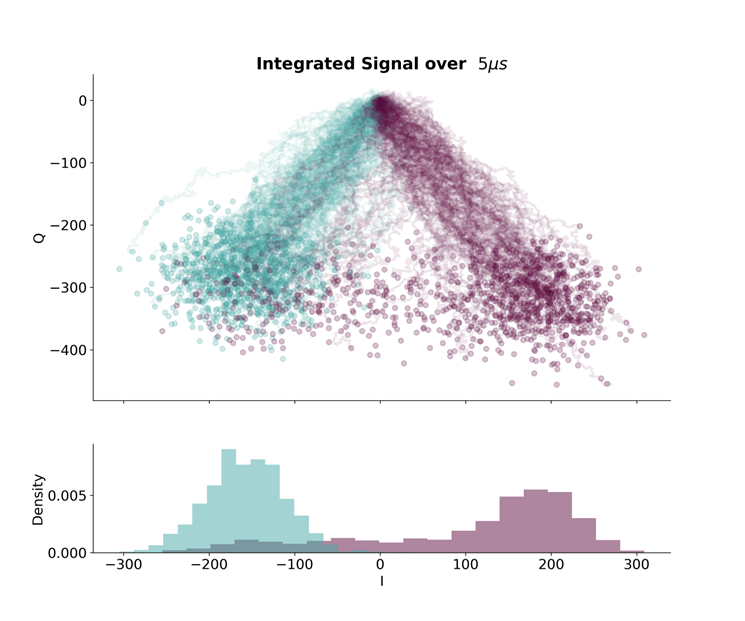
\includegraphics{Figs/Theory/stochastic_signal.png}
%     \caption{The trajectories given by driving a resonator in between the two peaks for $\ket{0}$ and $\ket{1}$ respectively.}
%     \label{fig:stochastic_signal_hetereodyne}
% \end{figure}
In heterodyne measurements, the signal is mixed in an IQ-mixer with a local oscillator. By delaying one part of local oscillator pulse with a phase of $\pi / 2$, it is possible to measure two quadrature components with half strength. The signals become:
\begin{align}
    V_0               &= A_{RO}A_{LO} \cos(\omega_{IF}t + \theta_{RO}) \\
    V_{\frac{\pi}{2}} &= A_{RO}A_{LO} \sin(\omega_{IF}t + \theta_{RO})
\end{align}
If we combine the two signals into a complex number, we can demodulate it by multiplying with $e^{-i\omega_{IF}t}$:
\begin{equation}
    V(t) = e^{-i\omega_{IF} t} (V_0 + i V_{\frac{\pi}{2}}) = A_{RO} e^{i\theta_{RO}}
\end{equation}
Thus we at each timestep get a signal in the complex plane. 

The corresponding operators to this process, can be thought of by splitting the Heterodyne measurement in two Homodyne processes with half the signal each. Such that we have
\begin{equation}
    c_0 = \sqrt{\frac{\kappa}{2}}\; a, \quad c_{\frac{\pi}{2}} = i \sqrt{\frac{\kappa}{2}} \; a
\end{equation}
Which we can model as two inefficient observers, where we keep the information of both of them. Combining the two records into a complex number leads to
\begin{equation}
    dr_{\text{heterodyne}}(t) = \left(\expval{I} + i\expval{Q}\right)dt  + \frac{1}{\sqrt{2\eta\kappa}}(dW_I + i dW_Q)
\end{equation}
Where we have associated the two quadratures with $I$ and $Q$. Both of which come with a noise process. However, we should still notice that $\mathcal{D}[a] = \mathcal{D}[ia]$ such that applying the hetereodyne measurement leads to the same dissipation as in the homodyne case. This also makes sense since it is the same signal we look at, we just split it in two. 
%\footnote{since $\mathcal{D}[ia] \rho = ia\rho (-ia^\dagger) - \frac12 \left(-ia^\dagger ia \rho + \rho (-ia^\dagger ia\right) = \mathcal{D}[a]$ when canceling the $i \cdot (-i) = 1$ factors}


\section{Measurement Induced Backaction on the Qubit}\label{sec:qubit_backaction}
The section above, does not directly measure the qubit, but is indirectly measuring it by determining the state of the resonator. It is however possible\footnote{but difficult} to see how the measurements interact with the qubit, if we trace the out the resonator. In section \ref{sec:driving_resonator_iq_plane}, we considered how the resonator coherent states: $\alpha_g, \alpha_e$ associated with $\ket{0}$ and $\ket{1}$ behaves under dispersive readout. 

The idea is to use the transformation $P = \ket{g}\bra{g}D(\alpha_g) + \ket{e}\bra{e}D(\alpha_e)$ where $D(\alpha)$ is the displacement operator moving the coherent state with an amount $\alpha$ in phase space. By applying this transformation, the dynamics are moved from the resonator and unto the qubit such that we can trace out the resonator and see how the qubit is affected \cite{gambetta_quantum_2008}. 
By transforming the Hamiltoninan, and tracing out the resonator, before doing the inverse transformation of the qubit. Gambetta et al. finds that the qubit experiences an effective frequency shift by:
\begin{equation}
    \omega_Q \to \omega_Q + 2 \chi \Re[\alpha_g(t)\alpha_e^*(t)]
\end{equation}
In addition, the resonator decay also affects the qubit with a dephasing term. $\mathcal{D}[a]\rho$ will in this transformation lead to a qubit interaction according to:
\begin{equation}
    \kappa\mathcal{D}(a) \to 2\chi \Im[\alpha_g(t)\alpha_e^*(t)] \mathcal{D}[\sigma_z]
\end{equation}
Where the corresponding backaction from the measurement will take the form of \cite{campagne-ibarcq_measurement_nodate}:
\begin{equation}
    \eta\mathcal{H}(\sqrt{\kappa} a) \to \eta \sqrt{2 \chi \Im[\alpha_g(t)\alpha_e^*(t)]} \mathcal{H}[\sigma_z]
\end{equation}
The equation allow us to see how the qubit is dephased by our measurements. Further, we get an additional approximation, where we can average out the resonator in the dispersive limit, under the further assumption that both the state of the resonator will be coherent when starting from a both $\ket{0}$ and $\ket{1}$. While this significantly reduces the complexity of the simulation\footnote{since the resonator accounts for the largest part of the Hilbert Space}. An example is is that $T_1$ is not modelled well by these equations \footnote{In \cite{gambetta_quantum_2008} the transformation is done with the assumption that $T_1 \gg 1 / \kappa$}. 